% ============================================================================
% TriangleFX -- CSC360 Group 1 -- Beamer presentation (10 slides)
% Build:  pdflatex TriangleFX_Presentation.tex   (run twice for the outline)
% ============================================================================
\documentclass[aspectratio=169,11pt]{beamer}

\usepackage[utf8]{inputenc}
\usepackage[T1]{fontenc}
\usepackage{lmodern}
\usepackage{amsmath,amssymb}
\usepackage{booktabs}
\usepackage{tabularx}
\usepackage{listings}
\usepackage{tikz}
\usetikzlibrary{arrows.meta,positioning,shapes.geometric,calc,fit}

% ---------------------------------------------------------------- theme ----
\usetheme{Madrid}
\definecolor{tfxbg}{HTML}{0F172A}
\definecolor{tfxpanel}{HTML}{1E293B}
\definecolor{tfxblue}{HTML}{2563EB}
\definecolor{tfxsky}{HTML}{58A6FF}
\definecolor{tfxred}{HTML}{DC2626}
\definecolor{tfxgreen}{HTML}{16A34A}
\definecolor{tfxamber}{HTML}{D97706}
\setbeamercolor{palette primary}{bg=tfxbg,fg=white}
\setbeamercolor{palette secondary}{bg=tfxpanel,fg=white}
\setbeamercolor{palette tertiary}{bg=tfxblue,fg=white}
\setbeamercolor{title}{fg=white,bg=tfxbg}
\setbeamercolor{frametitle}{bg=tfxbg,fg=white}
\setbeamercolor{structure}{fg=tfxblue}
\setbeamercolor{block title}{bg=tfxblue,fg=white}
\setbeamercolor{block body}{bg=tfxblue!8,fg=black}
\setbeamercolor{block title alerted}{bg=tfxred,fg=white}
\setbeamercolor{block body alerted}{bg=tfxred!8,fg=black}
\setbeamercolor{block title example}{bg=tfxgreen,fg=white}
\setbeamercolor{block body example}{bg=tfxgreen!8,fg=black}
\setbeamertemplate{navigation symbols}{}
\setbeamertemplate{itemize items}[circle]

\lstset{
  basicstyle=\ttfamily\scriptsize,
  keywordstyle=\color{tfxblue}\bfseries,
  commentstyle=\color{gray}\itshape,
  stringstyle=\color{tfxamber},
  language=Java,
  showstringspaces=false,
  breaklines=true,
  frame=single,
  rulecolor=\color{tfxblue!40},
  backgroundcolor=\color{gray!6},
  morekeywords={record,var}
}

\title[TriangleFX]{TriangleFX}
\subtitle{From Three Equations to a Valid Triangle}

\author[CSC360 Group 1]{}
\institute[]{}
\date{}

\begin{document}

% ---------------------------------------------------------------- 1 -------
\begin{frame}[plain]

    % ---------- Title ----------
    \begin{beamercolorbox}[
        wd=\paperwidth,
        sep=10pt,
        center
    ]{title}
        {\usebeamerfont{title}\inserttitle\par}
        \vspace{4pt}
        {\usebeamerfont{subtitle}\insertsubtitle\par}
    \end{beamercolorbox}

    \vspace{0.45cm}

    % ---------- Objective ----------
    \begin{block}{Objective}
        \small
        Create a JavaFX application that takes three equations, finds where the lines meet, checks if they form a valid triangle, and displays the triangle on the screen.
    \end{block}

    \vfill

    % ---------- Bottom section ----------
    \begin{columns}[T]

        % ----- Left: Team -----
        \begin{column}{0.48\textwidth}
            \textbf{Group 1}

            \vspace{0.15cm}

            \begin{tabular}{ll}
                Devang Parmar  & AU2340217 \\
                Dhairya Rupani & AU2340195 \\
                Vidhan Nahar   & AU2340199 \\
                Drumil Bhati   & AU2340211
            \end{tabular}
        \end{column}

        % ----- Right: Course -----
        \begin{column}{0.48\textwidth}
            \raggedleft
            \textbf{Mentor}\\
            Professor Susanta Tewari

            \vspace{0.25cm}

            \textbf{Course}\\
            CSC360 Computer Graphics and Digital Image Processing
        \end{column}

    \end{columns}

\end{frame}

% ---------------------------------------------------------------- 2 -------
\begin{frame}{1. Problem Statement}

  \begin{columns}[T]

    % ------------------------------------------------
    % LEFT COLUMN
    % ------------------------------------------------
    \column{0.52\textwidth}

      \begin{block}{The Problem}
        We are given \textbf{three equations} representing three lines.
        Our goal is to find where the lines meet and determine whether
        they form a valid triangle.
      \end{block}

      \vspace{4pt}

      \textbf{What the system does:}

\begin{itemize}
    \item Takes three equations as input
    \item Finds the three intersection points
    \item Checks if the intersection points form a triangle
    \item Calculates area, perimeter, sides and centroid
    \item Draws the triangle on a coordinate plane
\end{itemize}

    % ------------------------------------------------
    % RIGHT COLUMN
    % ------------------------------------------------
    \column{0.44\textwidth}

      \begin{alertblock}{When is it Invalid?}
        \begin{itemize}
          \item Two lines are parallel
          \item Two lines are the same
          \item All three lines meet at one point
          \item The three intersection points lie on one line
          \item Input is missing or invalid
        \end{itemize}
      \end{alertblock}

      \begin{exampleblock}{Example} $x+y=8,\; x-y=2,\; x=1$\\[2pt] $\Rightarrow$ vertices $(5,3),(1,-1),(1,7)$ \end{exampleblock}

  \end{columns}

\end{frame}

% ---------------------------------------------------------------- 3 -------
\begin{frame}{2. Thought Process}

  \begin{center}
  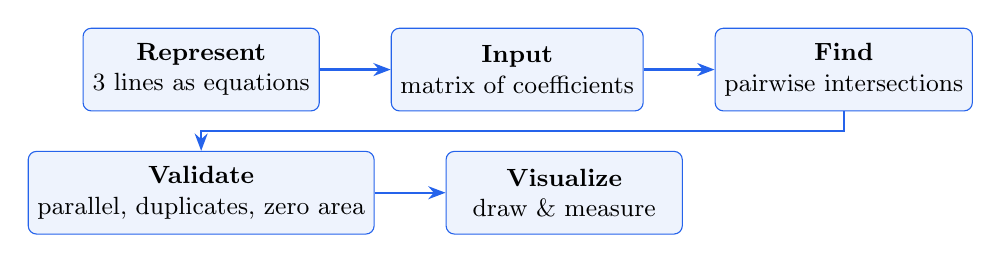
\begin{tikzpicture}[
      node distance=5mm and 9mm,
      pstep/.style={
        draw=tfxblue,
        fill=tfxblue!8,
        rounded corners=3pt,
        align=center,
        minimum width=3.0cm,
        minimum height=1.05cm,
        font=\small
      },
      arr/.style={
        -{Stealth[length=2.2mm]},
        thick,
        tfxblue
      }
    ]

    \node[pstep] (a)
      {\textbf{Represent}\\3 lines as equations};

    \node[pstep,right=of a] (b)
      {\textbf{Input}\\matrix of coefficients};

    \node[pstep,right=of b] (c)
      {\textbf{Find}\\pairwise intersections};

    \node[pstep,below=of a] (d)
      {\textbf{Validate}\\parallel, duplicates, zero area};

    \node[pstep,right=of d] (e)
      {\textbf{Visualize}\\draw \& measure};

    \draw[arr] (a)--(b);
    \draw[arr] (b)--(c);

    \draw[arr]
  (c.south) -- ++(0,-2.5mm)
  -| ($(d.north)+(0,0)$);

    \draw[arr] (d)--(e);

  \end{tikzpicture}
  \end{center}

  \vspace{-2mm}

  \begin{columns}[T]

    \column{0.48\textwidth}

      \textbf{Principles}

      \begin{itemize}
        \item Represent the three lines using a structured
              \textbf{3$\times$2 matrix + 3 constants}
        \item Keep mathematical logic \textbf{separate from the UI}
        \item Treat invalid geometry as an expected outcome
      \end{itemize}

    \column{0.48\textwidth}

      \textbf{How We Built It}

      \begin{itemize}
        \item Support direct matrix input and predefined presets
        \item Solve each pair of lines independently
        \item Automatically scale the canvas to display the triangle
      \end{itemize}

  \end{columns}

\end{frame}

% ---------------------------------------------------------------- 4 -------
\begin{frame}{3. The Mathematics}
  \begin{columns}[T]
    \column{0.48\textwidth}
      \begin{block}{1. Matrix Formulation ($A\mathbf{x} = \mathbf{b}$)}
        \[
          \begin{bmatrix} a_{11} & a_{12} \\ a_{21} & a_{22} \\ a_{31} & a_{32} \end{bmatrix}
          \begin{bmatrix} x \\ y \end{bmatrix} =
          \begin{bmatrix} b_1 \\ b_2 \\ b_3 \end{bmatrix}
          \quad \begin{subarray}{l} \text{\scriptsize Line 1} \\ \text{\scriptsize Line 2} \\ \text{\scriptsize Line 3} \end{subarray}
        \]
      \end{block}
      \vspace{2pt}
      \begin{block}{2. Vertex Intersection (Cramer's Rule)}
        \footnotesize
        For lines $L_1, L_2$ ($D = a_{11}a_{22} - a_{21}a_{12} \neq 0$):
        \[
          x = \frac{b_1 a_{22} - b_2 a_{12}}{D}, \quad
          y = \frac{a_{11} b_2 - a_{21} b_1}{D}
        \]
        Gives corners $P_{12}, P_{23}, P_{31}$ ($D=0 \implies \text{parallel}$).
      \end{block}

    \column{0.48\textwidth}
      \begin{block}{3. Triangle Properties}
        \footnotesize
        \textbf{Area (Shoelace):} $\Delta = \tfrac{1}{2}\bigl|x_1(y_2-y_3) + x_2(y_3-y_1) + x_3(y_1-y_2)\bigr|$\\[4pt]
        \textbf{Centroid (Balance):} $G = \bigl(\tfrac{x_1 + x_2 + x_3}{3}, \, \tfrac{y_1 + y_2 + y_3}{3}\bigr)$\\[4pt]
        \textbf{Perimeter:} $p = a + b + c \quad (d = \sqrt{\Delta x^2 + \Delta y^2})$
      \end{block}
      \vspace{4pt}
      \begin{exampleblock}{4. Geometric Validation}
        \footnotesize
        \textbf{Valid} $\iff D \neq 0$, distinct corners, and $\Delta \ge 10^{-6}$.\\[1pt]
        \scriptsize (Rejects parallel, coincident, concurrent, or flat lines)
      \end{exampleblock}
  \end{columns}
\end{frame}
    

% ---------------------------------------------------------------- 5 -------
\begin{frame}{4. The Solution: Layered Architecture}
  \centering
  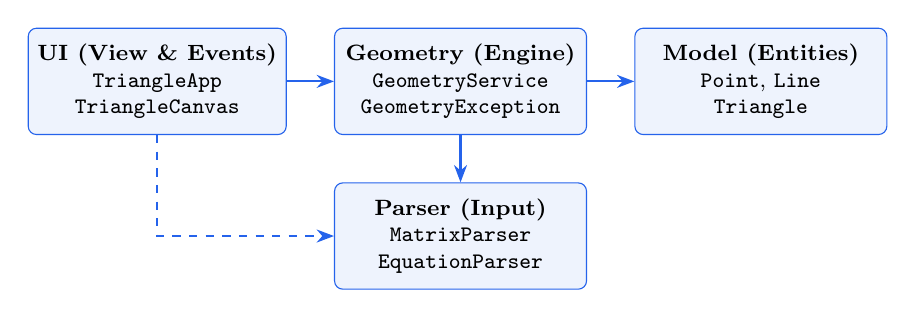
\begin{tikzpicture}[
      node distance=6mm,
      layer/.style={draw=tfxblue,fill=tfxblue!8,rounded corners=3pt,align=center,
                    minimum width=3.2cm,minimum height=1.35cm,font=\footnotesize},
      arr/.style={-{Stealth[length=2.2mm]},thick,tfxblue}]
    \node[layer] (ui)    {\textbf{UI (View \& Events)}\\ \texttt{TriangleApp}\\ \texttt{TriangleCanvas}};
    \node[layer,right=of ui]    (svc)   {\textbf{Geometry (Engine)}\\ \texttt{GeometryService}\\ \texttt{GeometryException}};
    \node[layer,right=of svc]   (model) {\textbf{Model (Entities)}\\ \texttt{Point}, \texttt{Line}\\ \texttt{Triangle}};
    \node[layer,below=of svc]   (parse) {\textbf{Parser (Input)}\\ \texttt{MatrixParser}\\ \texttt{EquationParser}};
    \draw[arr] (ui)--(svc);
    \draw[arr] (svc)--(model);
    \draw[arr] (svc)--(parse);
    \draw[arr,dashed] (ui.south) |- (parse.west);
  \end{tikzpicture}

  \vspace{1mm}
  \begin{columns}[T]
    \column{0.48\textwidth}
      \begin{block}{Architecture Principles}
        \footnotesize
        \begin{itemize}\setlength{\itemsep}{2pt}\setlength{\parskip}{0pt}
          \item \textbf{Decoupled Core:} Math in \texttt{model}/\texttt{geometry} has zero JavaFX UI dependencies.
          \item \textbf{Separation of Concerns:} UI renders; Parser sanitizes; Geometry validates.
        \end{itemize}
      \end{block}

    \column{0.48\textwidth}
      \begin{block}{Key Engineering Benefits}
        \footnotesize
        \begin{itemize}\setlength{\itemsep}{2pt}\setlength{\parskip}{0pt}
          \item \textbf{Headless Testing:} All math is 100\% testable with JUnit without a display.
          \item \textbf{Clear Failure Feedback:} Custom exceptions explain invalid geometry in the UI.
        \end{itemize}
      \end{block}
  \end{columns}
\end{frame}
% ---------------------------------------------------------------- 6 -------
\begin{frame}[fragile]{5. Solution Walk-through: Validation Pipeline}
  \begin{columns}[T]
    \column{0.41\textwidth}
      \small
      \textbf{Fail-Fast Validation Pipeline:}
      \begin{enumerate}\setlength{\itemsep}{0.5pt}\setlength{\parskip}{0pt}
        \item \textbf{Pairwise check}: Reject parallel ($D=0$) or coincident lines.
        \item \textbf{Cramer's intersection}: Compute vertices $(P_{12}, P_{23}, P_{31})$.
        \item \textbf{Concurrency check}: If $P_{12} \approx P_{23}$, lines cross at 1 point ($\epsilon = 10^{-6}$).
        \item \textbf{Collinearity / Area}: Reject flat triangle if $\Delta < 10^{-6}$.
        \item Return immutable \texttt{Triangle}.
      \end{enumerate}
      \vspace{1pt}
      \begin{alertblock}{Defensive Engineering}
        \footnotesize
        Eliminates division-by-zero ($D=0$) early; tolerances protect against IEEE-754 precision limits.
      \end{alertblock}

    \column{0.57\textwidth}
\begin{lstlisting}[basicstyle=\ttfamily\fontsize{5.5}{6.8}\selectfont,breaklines=false,xleftmargin=1pt,xrightmargin=1pt]
public Triangle buildTriangle(Line l1, Line l2, Line l3)
    throws GeometryException {
  // 1. Fail-fast: reject parallel / identical pairs
  checkPair(l1, l2, 1, 2);
  checkPair(l2, l3, 2, 3);
  checkPair(l3, l1, 3, 1);

  // 2. Pairwise intersection via Cramer's rule
  Point p12 = l1.intersectionWith(l2).orElseThrow();
  Point p23 = l2.intersectionWith(l3).orElseThrow();
  Point p31 = l3.intersectionWith(l1).orElseThrow();

  // 3. Concurrency check (tolerance = 1e-6)
  if (p12.equalsWithTolerance(p23, TOL) ||
      p23.equalsWithTolerance(p31, TOL) ||
      p31.equalsWithTolerance(p12, TOL)) {
    throw new GeometryException("Lines are concurrent.");
  }

  // 4. Area threshold check (reject degenerate/flat)
  Triangle t = new Triangle(p12, p23, p31, l1, l2, l3);
  if (t.getArea() < MIN_AREA) {
    throw new GeometryException("Collapsed triangle.");
  }
  return t;
}
\end{lstlisting}
  \end{columns}
\end{frame}

% ---------------------------------------------------------------- 7 -------
\begin{frame}{6. Rendering: World-to-Screen Mapping}
  \begin{columns}[T]
    \column{0.52\textwidth}
      \small
      \textbf{Window-to-Viewport Transformation}
      \begin{itemize}\setlength{\itemsep}{1pt}\setlength{\parskip}{0pt}
        \item \textbf{World Space}: $(0,0)$ Cartesian center, $+y$ points \textbf{UP}
        \item \textbf{Screen Space}: $(0,0)$ Top-Left corner, $+y$ points \textbf{DOWN}
      \end{itemize}
      \[
        X_{\text{px}} = \tfrac{W}{2} + (x - x_c)\cdot s, \quad
        Y_{\text{px}} = \tfrac{H}{2} - (y - y_c)\cdot s
      \]
      \textbf{Uniform Scaling \& Margins (Aspect 1:1)}:
      \[
        s = \min\left(\frac{W - 80}{\text{span}_x \cdot 1.7}, \; \frac{H - 80}{\text{span}_y \cdot 1.7}\right)
      \]
      \vspace{-2pt}
      \begin{block}{Painter's Algorithm Pipeline}
        \footnotesize
        Grid $\to$ Axes $\to$ Extended Dashed Lines $\to$ Alpha Fill ($\alpha=0.25$) $\to$ Stroke $\to$ Vertex Badges (radial offset).
      \end{block}

    \column{0.46\textwidth}
      \begin{center}
      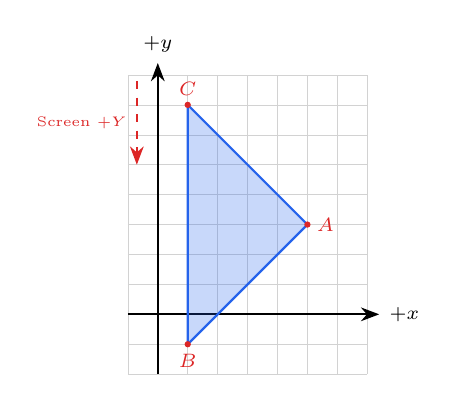
\begin{tikzpicture}[scale=0.38,>=Stealth]
        \draw[step=1,gray!35,very thin] (-1,-2) grid (7,8);
        \draw[->,thick] (-1,0)--(7.4,0) node[right]{\scriptsize $+x$};
        \draw[->,thick] (0,-2)--(0,8.4) node[above]{\scriptsize $+y$};
        \draw[->,dashed,tfxred,thick] (-0.7,7.8)--(-0.7,5.0) node[midway,left]{\tiny Screen $+Y$};
        \fill[tfxblue,opacity=0.25] (5,3)--(1,-1)--(1,7)--cycle;
        \draw[tfxblue,thick] (5,3)--(1,-1)--(1,7)--cycle;
        \foreach \p/\l/\pos in {(5,3)/A/right,(1,-1)/B/below,(1,7)/C/above}
          \fill[tfxred] \p circle(3pt) node[\pos]{\scriptsize $\l$};
      \end{tikzpicture}

      \vspace{2pt}
      {\scriptsize Vertices: $A(5,3),\,B(1,-1),\,C(1,7)$ (radial label offset from $G$)}
      \end{center}
  \end{columns}
\end{frame}

% ---------------------------------------------------------------- 8 -------
\begin{frame}{7. Design Patterns Used}
  \begin{columns}[T]
    \column{0.47\textwidth}
      \begin{block}{Facade}
        \textbf{Class:} \texttt{GeometryService}

        \vspace{4pt}
        \textbf{Method:} \texttt{buildTriangle(...)}

        \vspace{4pt}
        The UI calls this one method. It handles equation parsing,
        line intersections, and triangle validation.
      \end{block}

      \vspace{6pt}
      \begin{exampleblock}{Call from the UI}
        \texttt{service.buildTriangle(eq1, eq2, eq3)}
      \end{exampleblock}

    \column{0.47\textwidth}
      \begin{block}{Observer}
        \textbf{Class:} \texttt{TriangleCanvas}

        \vspace{4pt}
        \textbf{Observed values:} canvas width and height

        \vspace{4pt}
        When the window size changes, JavaFX notifies the
        canvas. The canvas then calls \texttt{redraw()}.
      \end{block}

      \vspace{6pt}
      \begin{exampleblock}{Listener in the code}
        \texttt{widthProperty().addListener(...)}\\
        \texttt{heightProperty().addListener(...)}
      \end{exampleblock}
  \end{columns}
\end{frame}

% ---------------------------------------------------------------- 9 -------
\begin{frame}{8. Tests}
  \begin{columns}[T]
    \column{0.50\textwidth}
      \begin{block}{GeometryServiceTest}
        \begin{itemize}
          \item Builds a triangle from equations
          \item Builds a triangle from a matrix
          \item Rejects invalid matrix sizes
          \item Rejects parallel, identical, and concurrent lines
          \item Checks a right triangle
        \end{itemize}
      \end{block}
      \begin{block}{What these tests check}
        The geometry service returns the expected points and measurements
        for valid input, and reports an error for invalid input.
      \end{block}
    \column{0.46\textwidth}
      \begin{exampleblock}{EquationParserTest}
        \begin{itemize}
          \item Reads standard equations
          \item Reads vertical and horizontal lines
          \item Reads decimal and negative values
          \item Rejects invalid equations
        \end{itemize}
      \end{exampleblock}
      \begin{exampleblock}{MatrixParserTest}
        \begin{itemize}
          \item Reads both supported matrix formats
          \item Rejects the wrong number of values
        \end{itemize}
      \end{exampleblock}
  \end{columns}
\end{frame}

% --------------------------------------------------------------- 10 -------
\begin{frame}{9. Reference Material, Lessons and Next Steps}
  \small
  \begin{columns}[T]
    \column{0.52\textwidth}
      \textbf{Reference books (\texttt{Books/})}
      \begin{itemize}
        \item \emph{Core Java, Vol.~1 \& 2}: classes, immutability, exceptions, regular expressions
        \item \emph{Introducing JavaFX 8 Programming} (Weaver): scene graph, \texttt{Canvas}, property listeners
        \item \emph{Graphics with Java} (2007): 2D drawing and coordinate transformations
        \item \emph{Digital Image Processing} (Burger \& Burge): geometric coordinate mapping
      \end{itemize}
    \column{0.44\textwidth}
      \textbf{Lessons learned}
      \begin{itemize}
        \item Fix the input model first
        \item Floating point needs explicit tolerances
        \item Domain exceptions give clear UI messages
      \end{itemize}
      \textbf{Next steps}
      \begin{itemize}
        \item Property-based tests
        \item Export drawing as PNG/SVG
        \item Generalise to $n$ lines
      \end{itemize}
  \end{columns}
  \vspace{2mm}
  \centering
  {\large\color{tfxblue}\textbf{Thank you --- Questions?}}
\end{frame}

\end{document}
